\documentclass[conference]{IEEEtran}
\IEEEoverridecommandlockouts

\usepackage{cite}
\usepackage{amsmath,amssymb,amsfonts}
\usepackage{graphicx}
\usepackage{textcomp}
\usepackage{xcolor}
\usepackage{booktabs}
\usepackage{microtype}
\usepackage{orcidlink}
\usepackage{tikz}
\usetikzlibrary{shapes.geometric,arrows.meta,positioning,fit,calc,decorations.pathreplacing}
\usepackage[section]{placeins}
\usepackage{hyperref}   % load last; subsumes the url package
\def\UrlBreaks{\do\/\do-\do_\do.\do=\do?\do&\do\#}
\hypersetup{
  colorlinks=true,
  linkcolor=black,
  citecolor=black,
  urlcolor=black
}

\newcommand{\sys}{Project Simurgh}

\begin{document}

\title{Privacy-Preserving Integrity Evidence for\\Student-Society Voting-Adjacent Workflows:\\
A Phase C Pilot of \sys{} at Macquarie University%
\thanks{Voting-adjacent case study, not a production election-security claim.
Research prototype only. Source:
\url{https://github.com/Raoof128/Project-Simurgh}~\cite{simurgh2026}.
Tag: \texttt{v0.5.0-voting-pilot-phase-c-closeout}.
DOI:~\href{https://doi.org/10.5281/zenodo.20549736}{10.5281/zenodo.20549736}~\cite{abedini2026votingpilot}.}}

\author{
  \IEEEauthorblockN{Mohammad Raouf Abedini\,\orcidlink{0009-0000-6214-258X}}
  \IEEEauthorblockA{
    \textit{Department of Computing}\\
    Macquarie University\\
    Sydney, Australia\\
    mohammadraouf.abedini@students.mq.edu.au\\
    \url{https://raoufabedini.dev}
  }
}

\maketitle

%% ── ABSTRACT ──────────────────────────────────────────────────────────────
\begin{abstract}
In a Phase~C pilot of 31 consented sessions (30 submitted, 1 withdrawn)
alongside a real student-society voting event, a consent-based shadow-mode
system collected session-integrity metadata without recording ballot choices.
This boundary was enforced through explicit submit-call JSON construction,
client-side ballot-field exclusion safeguards, and server-side
forbidden-field rejection, rather than by policy alone.
Existing cryptographic schemes primarily address outcome integrity, while the
telemetry-collection question studied here is narrower: whether a shadow-mode
system can produce evidence that it collected only what it disclosed.
\sys{} addresses this question with an HMAC-SHA-256 audit chain~\cite{rfc2104},
a server-side forbidden-field guard, and a collection-closure flag that returns
\texttt{HTTP~410 Gone} on all write routes once data collection ends.
The report builder emits
\texttt{ballot\_choice\_recorded\_by\_simurgh: false}
as an implementation-enforced invariant; the closeout gate suite verified this
invariant after the 30 submitted sessions: 359/359 automated tests, 8/8 smoke
gates, 10/10 security-audit gates, and 5/5 closure gates passed at closeout.
This study is voting-adjacent: it does not implement ballot cryptography,
eligibility verification, coercion resistance, tally protection, or
public-election certification; the ballot-choice exclusion boundary is
enforced by structural design, not participant behavior.
\end{abstract}

\begin{IEEEkeywords}
data privacy, message authentication, audit trails, electronic voting,
consent management, student governance
\end{IEEEkeywords}

%% ── I. INTRODUCTION ───────────────────────────────────────────────────────
\section{Introduction}

Digital voting tools support event preference polls, committee elections, and
budget decisions in student societies, including at Macquarie University where
this pilot was conducted. These tools leave a gap that existing cryptographic
solutions do not address: session integrity in the presence of a potential
covert collector: whether the system collected only what it disclosed, and
no more.

End-to-end verifiable voting schemes~\cite{adida2008helios,clarkson2008civitas}
solve the \emph{outcome} integrity problem (did the tally reflect all ballots?)
but do not address \emph{session} integrity (was the participant's interaction
free of covert collection?). \sys{} is a research prototype that targets session
integrity through privacy-preserving metadata collection and tamper-evident
audit chains~\cite{simurgh2026}. It was developed in response to the Invisible
Window attack~\cite{abedini2026invisible}, which demonstrated that OS-level
display affinity APIs allow application windows to evade browser-based screen
capture entirely, undermining the display-fidelity assumption on which WebRTC
proctoring relies. This paper is a companion to the main \sys{} architecture
paper~\cite{simurgh2026}; it reports the Phase~C voting-adjacent pilot as a
bounded, application-specific case study of that system.

This paper reports a Phase~C pilot in which \sys{} ran in shadow mode alongside
a real MQ Persian Society event preference poll, collecting session-level
integrity metadata in parallel with no effect on the official result. We use
\emph{voting-adjacent} to mean the system ran entirely separate from the
official ballot-counting infrastructure, with no access to ballot choices or
influence on official outcomes. The pilot was not a study of election security,
voting-system integrity, or electoral fraud prevention.

\medskip
\noindent\textbf{Contributions:}
\begin{itemize}
  \item A consent-to-submit pilot with 30 submitted sessions verifying
    \texttt{ballot\_choice\_recorded\_by\_simurgh: false} as an
    implementation-enforced invariant in every session, backed by smoke,
    security-audit, and privacy-audit gate suites (Sec.~\ref{sec:results}).
  \item A verifiable end-of-collection posture in which the collection-closed
    middleware executes before authentication on all write routes, preventing
    token-bearing clients from bypassing closure and verifiable at the API
    layer by any caller able to reach the pilot endpoint
    (Sec.~\ref{sec:design}).
  \item A gate-verified evidence methodology pairing implementation-enforced
    structural invariants with independently runnable smoke, security-audit,
    and privacy-audit suites, archived at tag
    \texttt{v0.5.0-voting-pilot-phase-c-closeout} for reproducing the
    implementation-enforced gate checks and extending the methodology to future
    privacy-preserving integrity evidence work in voting-adjacent contexts.
\end{itemize}

%% ── II. RELATED WORK ──────────────────────────────────────────────────────
\section{Related Work}

\subsection{End-to-End Verifiable Voting}

Systems such as Helios~\cite{adida2008helios} use homomorphic tallying or
mix-net shuffles so voters can verify their encrypted ballot was counted without
revealing the plaintext choice. Civitas~\cite{clarkson2008civitas} adds
coercion resistance; STAR-Vote~\cite{bell2013starvote} adds risk-limiting-audit
integration.

\sys{} differs in scope. It does not implement ballot encryption,
voter-verifiable tallying, or public election certification. Where end-to-end
verifiable voting proves the integrity of the \emph{outcome}, \sys{} studies
the integrity of the \emph{participation session}: whether the system collected
only what it disclosed and nothing more.

\subsection{Remote and Internet Voting Security}

Remote electronic voting introduces risks beyond ordinary web application
security: endpoint compromise, coercion, eligibility verification, ballot
secrecy, and tally integrity. NIST guidance~\cite{nistir7770} identifies threat
categories for remote electronic voting and recommends caution around
internet-connected election infrastructure. The National Academies
report~\cite{nationalacademies2018} emphasizes that vote collection, alteration,
destruction, counting, and reporting each require separate mitigations.

This pilot addresses none of those concerns. It is a student-society research
case study, not a production online-voting system.

\subsection{Voting Standards, Privacy, and Auditability}

The U.S.\ Election Assistance Commission adopted VVSG~2.0 in
2021~\cite{vvsg2021}, establishing updated requirements for privacy,
accessibility, auditability, and software independence in voting systems.
Modern voting-system guidance consistently requires audit records that do not
reveal individual ballot choices.

\sys{} aligns with this direction: the HMAC audit chain records session
lifecycle events without ballot content, but remains outside public-election
certification scope.

\subsection{Australian Technology-Assisted Voting}

Several Australian jurisdictions have piloted technology-assisted voting,
including iVote in New South Wales. The NSW Electoral Commission's
technology-assisted voting review~\cite{nswec2023tav} examined privacy,
accessibility, and security trade-offs, recommending careful scoping and
ongoing evaluation before broader deployment. The NSW Electoral Commission's evidence-driven approach makes small, bounded
pilots the appropriate vehicle for evaluating session-integrity mechanisms at
the consent-privacy boundary.

\subsection{Privacy-Preserving Telemetry and Data Minimization}

\sys{}'s ballot-field exclusion architecture follows data-minimization
principles~\cite{cavoukian2009privacy}: the system collects the minimum metadata
required for a session-integrity signal and structurally prevents ballot-choice
data from reaching the server. Data that is structurally excluded from the
server cannot be leaked by the server; residual metadata (e.g., submission
timestamps) are minimized and out of scope for ballot-choice inference. The
contribution is not a new voting protocol; it is evidence that shadow-mode
session-integrity collection is achievable at student-governance scale without
access to ballot choices or influence on official outcomes.

%% ── III. SYSTEM DESIGN ────────────────────────────────────────────────────
\section{System Design}
\label{sec:design}

Fig.~\ref{fig:flow} shows the Phase~C session lifecycle.

\begin{figure}[t]
\centering
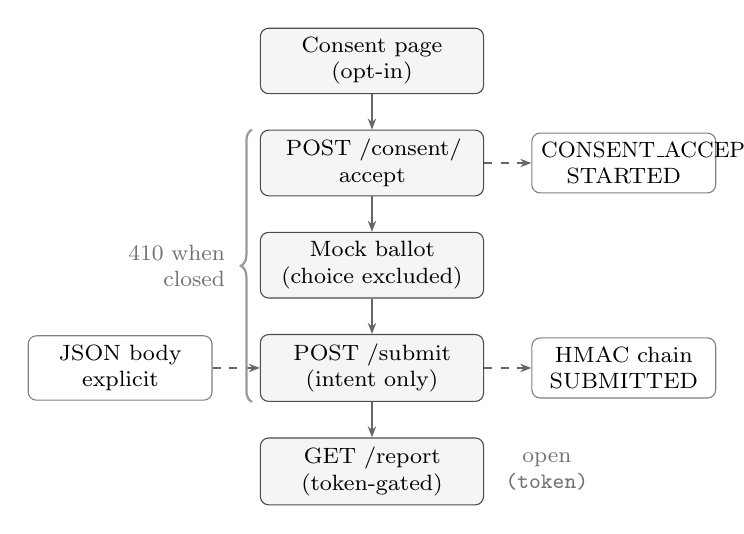
\begin{tikzpicture}[
  node distance=0.45cm and 0.1cm,
  box/.style={rectangle, rounded corners=3pt, draw=black!70, fill=gray!8,
              text width=2.6cm, align=center, font=\footnotesize,
              minimum height=0.7cm},
  act/.style={rectangle, rounded corners=3pt, draw=black!50, fill=white,
              text width=2.1cm, align=center, font=\footnotesize,
              minimum height=0.55cm},
  arr/.style={-{Stealth[length=4pt]}, thick, black!60},
  note/.style={font=\footnotesize, text=black!55, align=center}
]

%% Main flow nodes
\node[box] (consent) {Consent page\\(opt-in)};
\node[box, below=of consent] (accept) {POST /consent/\\accept};
\node[box, below=of accept]  (ballot)  {Mock ballot\\(choice excluded)};
\node[box, below=of ballot]  (submit)  {POST /submit\\(intent only)};
\node[box, below=of submit]  (report)  {GET /report\\(token-gated)};

%% Side annotation nodes
\node[act, right=0.6cm of accept] (chain1) {CONSENT\_ACCEPTED\\STARTED};
\node[act, right=0.6cm of submit] (chain2) {HMAC chain\\SUBMITTED};
\node[act, left=0.6cm of submit]  (discard) {JSON body\\explicit};

%% Main flow arrows
\draw[arr] (consent) -- (accept);
\draw[arr] (accept)  -- (ballot);
\draw[arr] (ballot)  -- (submit);
\draw[arr] (submit)  -- (report);

%% Side annotation arrows
\draw[arr, dashed] (accept)  -- (chain1);
\draw[arr, dashed] (submit)  -- (chain2);
\draw[arr, dashed] (discard) -- (submit);

%% Report annotation
\node[note, right=0.15cm of report] {open\\\texttt{(token)}};

%% 410-when-closed bracket
\draw[thick, black!40, decorate,
      decoration={brace, amplitude=4pt, mirror}]
  ([xshift=-0.1cm]accept.north west) -- ([xshift=-0.1cm]submit.south west)
  node[midway, left=6pt, font=\footnotesize, align=right, text=black!55]
    {410 when\\closed};

\end{tikzpicture}
\caption{Phase~C session lifecycle. The submit-call JSON body is constructed
explicitly without form serialization, so ballot data is structurally absent
(left). Two HMAC chain events append at consent (\texttt{CONSENT\_ACCEPTED},
\texttt{STARTED}) and one at submit (\texttt{SUBMITTED}) (right). Under the
collection-closed flag, write routes return \texttt{HTTP~410~Gone}; the report
endpoint remains token-protected.}
\label{fig:flow}
\end{figure}

\subsection{Consent Flow}

The consent page disclosed two categories: data \sys{} may collect across its
deployments (session timestamps, focus-loss and paste counts, audit-chain
validity signal, and an anonymous HMAC-hashed session code) and data it never
collects (ballot choices, screen recordings, webcam/audio, typed or pasted
content, raw process names, window titles, or device serial identifiers).
In Phase~C, implemented collection comprised only session timestamps,
audit-chain lifecycle events, and an anonymous participant code; focus-loss and
paste counts are exam-integrity features of the broader \sys{} system and were
not active in the voting pilot. This conservative disclosure posture means
participants consented to a superset of what was implemented.

On consent, the server issued an anonymous participant code and a signed session
token. No direct identifiers such as names, student identifiers, email
addresses, or ballot choices were collected.

\subsection{Ballot-Field Exclusion}

The submit handler constructed the JSON request body explicitly, containing only
\texttt{pilot\_session\_id} and \texttt{submit\_intent: true}; no form fields
were serialized into the body. As a future-code-change safeguard, the handler
also zeroed all radio button value properties (\texttt{el.value = ""}) before
the fetch call; this measure ensures ballot data cannot appear through a
form-serialization path if the construction were ever changed, though the
current implementation never serializes form fields. (The consent
\texttt{fetch} occurs before any ballot interaction and carries no ballot
field.) The server provided a second layer:
the \texttt{FORBIDDEN\_BALLOT\_FIELDS} set rejected any submission body
containing a known ballot-choice key with \texttt{HTTP~400}, with no echo of
the supplied value.

\subsection{HMAC Audit Chain}

Each session maintained an append-only HMAC-SHA-256 audit
chain~\cite{rfc2104} recording lifecycle events in sequence:
\texttt{CONSENT\_ACCEPTED} and \texttt{STARTED} (both appended at the
consent/accept call), then \texttt{SUBMITTED} at submit, and optionally
\texttt{BALLOT\_FIELD\_REJECTED}, \texttt{WITHDRAWN}, or
\texttt{REPORT\_EXPORTED}. The chain initialized on consent; the server
verified its integrity on report export.

\subsection{Collection-Closure Posture}

After reaching the 30-session target, we set the environment variable
\texttt{SIMURGH\_VOTING\_PILOT\_COLLECTION\_CLOSED} to \texttt{true}.
With this flag active:
\begin{itemize}
  \item \texttt{POST /api/voting-pilot/consent/accept} returns \texttt{410 Gone}.
  \item \texttt{POST /api/voting-pilot/submit} returns \texttt{410 Gone}.
  \item \texttt{POST /api/voting-pilot/withdraw} returns \texttt{410 Gone}.
  \item \texttt{GET /api/voting-pilot/:id/report} remains available,
    token-protected.
\end{itemize}
The closure middleware executes before authentication on write routes; a valid
session token cannot bypass it.

%% ── IV. PHASE C PILOT ─────────────────────────────────────────────────────
\section{Phase C Pilot}

\subsection{Study Design}

The pilot ran in shadow mode alongside the MQ Persian Society 2026 event
preference poll, asking members to select one of four proposed social events
(Nowruz cultural night, Persian movie night, career/networking night, food and
music night). \sys{} ran in parallel without access to or influence on the
official ballot-counting system. Each participant who joined the pilot completed
two steps: a consent page explaining data collection and a mock ballot page
mirroring the official event poll. The mock ballot choice was excluded from the
submit-call JSON body; \sys{} received only a submit-intent signal.

Participants were members of the society and were recruited through society
communication channels; participation was opt-in until the 30
submitted-session target was reached. Participation was voluntary and
governed by the Phase~C participant notice and data management addendum approved
by the society executive on 2026-06-04. No incentive was offered.
The society's official outcome was determined entirely outside \sys{}.
Session counts are reported in Table~\ref{tab:sessions}.

\subsection{Withdrawn Session}

One participant (\texttt{vp\_[redacted]}\footnote{Ephemeral pseudonymous token;
retained in the Phase~C closeout log.}) withdrew before submitting.
Withdrawn sessions are excluded from report export, privacy assertions, and
primary analysis; that session's report endpoint returns \texttt{HTTP~403}.

\subsection{Governance and Ethics}

Data collection was scoped to avoid directly identifying personal information
under the Privacy Act~1988~(Cth)~\cite{privacyact1988}: no names, student
identifiers, email addresses, ballot choices, demographic attributes, or
content-level data were collected. Because anonymous timestamps and session
metadata may still carry contextual privacy risk in a small cohort, this paper
reports only aggregate technical outcomes. No individual-level analysis,
disciplinary action, re-identification, or subgroup analysis was performed.
Participation was fully voluntary with no consequence for declining or
withdrawing. This paper does not claim formal institutional human-research ethics
approval; it reports a society-approved internal pilot with aggregate technical
outcomes only.

\subsection{Data Management}

The server held live session data in memory only. The application persisted no
live pilot session records; aggregate gate evidence and closeout artifacts were
separately archived in the repository. The store reset on server
restart, consistent with the data management addendum, which specified no
persistent storage of individual pilot session records.

%% ── V. RESULTS ────────────────────────────────────────────────────────────
\section{Results}
\label{sec:results}

\subsection{Dataset}

Phase~C recorded 31 consented pilot sessions, of which 30 completed the submit
step and formed the primary analysis dataset; one session was withdrawn before
submission. Table~\ref{tab:sessions} summarizes session counts.

The Phase~C human sessions are reported as aggregate closeout outcomes.
Individual live session records were not persisted; retained evidence consists
of closeout logs, gate outputs, source-level invariants, and the archived
implementation baseline at tag \texttt{v0.5.0-voting-pilot-phase-c-closeout}.

\begin{table}[!t]
  \caption{Session Counts---Phase~C Pilot}
  \centering
  \begin{tabular}{lr}
    \toprule
    Metric & Count \\
    \midrule
    Consented pilot sessions & 31 \\
    Submitted sessions (primary analysis) & 30 \\
    Withdrawn sessions & 1 \\
    \bottomrule
  \end{tabular}
  \label{tab:sessions}
\end{table}

\subsection{Privacy Assertions}

Table~\ref{tab:privacy} summarizes the privacy assertions across all 30 submitted sessions.

\begin{table}[!t]
  \caption{Privacy assertions across all 30 submitted sessions.
           (\texttt{ballot\_choice\_recorded} abbreviates
           \texttt{ballot\_choice\_recorded\_by\_simurgh}.)}
  \centering
  \begin{tabular}{ll}
    \toprule
    Assertion & Result \\
    \midrule
    \texttt{ballot\_choice\_recorded} & \texttt{false} \\
    \texttt{official\_vote\_impact}   & \texttt{false} \\
    Screen capture & No \\
    Webcam / audio & No \\
    Typed content & No \\
    Pasted content & No \\
    Personal device identifiers & No \\
    Raw process names & No \\
    Raw window titles & No \\
    Privacy audit (\texttt{privacy-audit.mjs}) & PASS \\
    \bottomrule
  \end{tabular}
  \label{tab:privacy}
\end{table}

The \texttt{ballot\_choice\_recorded\_by\_simurgh} field is a structural
guarantee: the value is hardcoded as \texttt{false} in the session report
builder and verified by the automated smoke suite at every gate run. Because the
session store was in-memory and cleared after collection, individual session
reports are not available post-hoc; the guarantee holds by implementation-enforced
design, not by retrospective per-session inspection. The privacy audit
(\texttt{privacy-audit.mjs}) performs static string-pattern searches across
source files and 52 pre-existing evidence export files to confirm the absence of
ballot-choice patterns in persisted data; Phase~C sessions were never persisted
and are therefore not included in that file count.

\subsection{Integrity Flow}

All 30 submitted sessions completed the consent-to-submit flow. The HMAC audit
chain recorded \texttt{CONSENT\_ACCEPTED} and \texttt{STARTED} on consent and
\texttt{SUBMITTED} on submit for each. The withdrawn session's chain recorded
\texttt{WITHDRAWN}; its report endpoint returned \texttt{HTTP~403}, confirming
exclusion from analysis.

\subsection{Safety Gates}

Table~\ref{tab:gates} shows all closeout gate results.

\begin{table}[!t]
  \caption{Safety Gates---Closeout Baseline}
  \centering
  \begin{tabular}{ll}
    \toprule
    Gate & Result \\
    \midrule
    Node tests (\texttt{npm test}) & 359/359 pass \\
    npm audit (\texttt{--audit-level=high}) & 0 high/critical \\
    Privacy audit & PASS (code + 52 evidence files) \\
    \texttt{smoke-voting-pilot.sh} & 8/8 pass \\
    \texttt{security-audit-voting-pilot.sh} & 10/10 pass \\
    \texttt{smoke-voting-pilot-closed.sh} & 5/5 pass \\
    \bottomrule
  \end{tabular}
  \label{tab:gates}
\end{table}

Gate evidence files are archived in the repository under the Phase~C closeout
evidence directory at tag \texttt{v0.5.0-voting-pilot-phase-c-closeout}.

\subsection{Collection Closure}

After collection reached 30 sessions, all write endpoints returned
\texttt{HTTP~410 Gone}. The closure smoke suite (5/5 gates) confirmed that
consent/accept, submit, and withdraw are unreachable under the closed
configuration, while report export remains available with a valid token,
verifiable at the API layer by any caller able to reach the pilot endpoint,
independently of the client UI state.

%% ── VI. DISCUSSION ────────────────────────────────────────────────────────
\section{Discussion}

\subsection{Interpretation}

The central finding is that structural enforcement, building privacy into the
system's data flow rather than relying on participant compliance, produces a
verifiable guarantee even without post-hoc per-session audit records. The
ballot-choice exclusion holds at the server layer regardless of client behavior
because the JSON body is constructed explicitly; browser-layer error or tampering
cannot introduce ballot data into an accepted submission, as attempts to include
ballot-choice fields are rejected by the server.
This makes the guarantee independent of participant trust, which matters for
adoption: a system that requires participants to trust both a policy and their
own correct behavior is weaker than one that enforces the boundary structurally.

The server-side collection-closure mechanism extends this approach: closure is
enforced at the infrastructure layer, specifically pre-authentication middleware,
and verifiable at the API layer by any caller able to reach the pilot endpoint.
Together, these design choices demonstrate a pattern applicable to any
shadow-mode telemetry deployment where the operator must demonstrate what was
and was not collected: both collection boundaries and collection closure can be
made API-observable and gate-verifiable.

\subsection{Limitations}

\begin{itemize}
  \item The 30-session dataset is a proof-of-concept pilot. No statistical
    power calculation was performed; results should not be generalized beyond
    this scope.
  \item Sessions were anonymous; no demographic or behavioral analysis of
    participants is possible or intended.
  \item The pilot ran in shadow mode only. No claim extends to a non-shadow
    deployment.
  \item The in-memory store means session data did not survive server restarts.
    This suits a research prototype but is not a production data-management
    posture.
  \item \texttt{ballot\_choice\_recorded\_by\_simurgh: false} is an
    implementation-enforced structural guarantee verified by the automated gate
    suite; per-session audit reports are not available post-hoc due to in-memory
    storage.
  \item The HMAC audit chain is keyed with a server-side secret; chain validity
    is operator-verifiable but not independently verifiable by participants
    without the signing key. This is consistent with the prototype scope but
    means the chain does not provide third-party attestation.
  \item The pilot was conducted in one student society at one university;
    results may not transfer to larger or more formal governance contexts.
  \item The pilot did not measure usability, accessibility, completion time,
    comprehension, or participant trust.
  \item The pilot did not include a formal adversarial participant study;
    malicious ballot-field attempts were tested through scripted security gates.
\end{itemize}

\subsection{Non-Claims}

This pilot does not claim to:
\begin{itemize}
  \item Secure or audit the official MQ Persian Society election result.
  \item Detect or prevent election fraud.
  \item Provide hardware-rooted attestation.
  \item Prevent or detect screen-capture evasion techniques (including
    display-affinity or GPU-layer approaches) on participant devices.
  \item Replace or improve the society's own voting system.
  \item Generalize to national, governmental, or binding elections.
\end{itemize}

%% ── VII. CONCLUSION ───────────────────────────────────────────────────────
\section{Conclusion}

Thirty sessions completed the full consent-to-submit flow in Phase~C of
\sys{}. In every session, the system collected no ballot choice, screen
recording, webcam or audio data, typed content, pasted content, or personal
device identifier. After data collection ended, all write endpoints returned
\texttt{HTTP~410 Gone} under a server-side flag, confirmed at the API layer
independently of the client UI by the 5/5 closure smoke suite.

The result demonstrates that privacy-preserving session-integrity evidence is
structurally achievable alongside a real student-society voting event. The
primary constraint for generalization is the operator-held HMAC signing
key: participant-verifiable integrity rather than operator-verifiable
integrity would require either a disclosed symmetric key or a public-key chain.
That extension, alongside a non-shadow deployment with a larger cohort, is the
natural next step for this research program.

%% ── REFERENCES ────────────────────────────────────────────────────────────
\bibliographystyle{IEEEtran}
\bibliography{references}

\end{document}
